\PassOptionsToPackage{usenames}{color}
\documentclass[11pt,a4paper]{article}

\usepackage{relsize} % relative font sizes (e.g. \smaller). must precede ACL style
\usepackage{style/acl2015}
\usepackage[colorlinks=true,linkcolor=black,citecolor=black,filecolor=black,urlcolor=black]{hyperref}
\usepackage{natbib}

%\usepackage{times}
%\usepackage{latexsym}

\usepackage{microtype}

\usepackage[boxed]{algorithm2e}
\renewcommand\AlCapFnt{\small}
\usepackage[small,bf,skip=5pt]{caption}
\usepackage{sidecap} % side captions
\usepackage{rotating}	% sideways
% \usepackage[pdftex]{graphicx}

% Italicize subparagraph headings
\usepackage{titlesec}
\titleformat*{\subparagraph}{\itshape}
\titlespacing{\subparagraph}{%
  1em}{%              left margin
  0pt}{% space before (vertical)
  1em}%               space after (horizontal)

% Numbered Examples and lists
\usepackage{lingmacros}
\newcommand{\exref}[1]{(\ref{#1})} % numbered example

\usepackage[shortlabels]{enumitem} % customizable lists
\setitemize{noitemsep,topsep=0em,leftmargin=*}
\setenumerate{noitemsep,leftmargin=0em,itemindent=13pt,topsep=0em}

\usepackage{xspace}
\usepackage{xparse} % for fancy custom macros (\NewDocumentEnvironment, etc.)

\newcommand{\indicator}[1]{\boldsymbol{1}\{#1\}}


\usepackage{textcomp}
% \usepackage{arabtex} % must go after xparse, if xparse is used!
%\usepackage{utf8}
% \setcode{utf8} % use UTF-8 Arabic
% \newcommand{\Ar}[1]{\RL{\novocalize #1}} % Arabic text

\usepackage{framed}

\usepackage{listings}

\lstset{
  basicstyle=\itshape,
  xleftmargin=3em,
  aboveskip=0pt,
  belowskip=-3pt, %-.5\baselineskip, % correct for extra paragraph break inserted after listing
  literate={->}{$\rightarrow$}{2}
           {α}{$\alpha$}{1}
           {δ}{$\delta$}{1}
           {(}{$($}{1}
           {)}{$)$}{1}
           {[}{$[$}{1}
           {]}{$]$}{1}
           {|}{$|$}{1}
           {+}{\ensuremath{^+}}{1}
           {*}{\ensuremath{^*}}{1}
}

\usepackage{amssymb}	%amsfonts,eucal,amsbsy,amsthm,amsopn
\usepackage{amsmath}

\usepackage{mathptmx}	% txfonts
\usepackage[scaled=.8]{beramono}
\usepackage[scaled=.85]{helvet}
\usepackage[T1]{fontenc}
\usepackage[utf8x]{inputenc}

\usepackage{MnSymbol}	% must be after mathptmx

\usepackage{latexsym}





% Tables
\usepackage{array}
\usepackage{multirow}
\usepackage{booktabs} % pretty tables
\usepackage{multicol}
\usepackage{footnote}
\newcolumntype{H}{>{\setbox0=\hbox\bgroup}c<{\egroup}@{}} % hidden column


\usepackage{url}
\usepackage[usenames]{color}
\usepackage{xcolor}

% colored frame box
\newcommand{\cfbox}[2]{%
    \colorlet{currentcolor}{.}%
    {\color{#1}%
    \fbox{\color{currentcolor}#2}}%
}

\usepackage[normalem]{ulem} % \uline
\usepackage{colortbl}
\usepackage{graphicx}
\usepackage{subcaption}
%\usepackage{tikz-dependency}
\usepackage{tikz}
%\usepackage{tree-dvips}
\usetikzlibrary{arrows,positioning,calc} 

\DeclareMathOperator*{\argmax}{arg\,max}
\DeclareMathOperator*{\argmin}{arg\,min}
%\setlength\titlebox{6.5cm}    % Expanding the titlebox
\setlength\titlebox{5.5cm}    % Expanding the titlebox

\usepackage{nameref}
\usepackage{cleveref}

% use \S for all references to all kinds of sections, and \P to paragraphs
% (sadly, we cannot use the simpler \crefname{} macro because it would insert a space after the symbol)
\crefformat{part}{\S#2#1#3}
\crefformat{chapter}{\S#2#1#3}
\crefformat{section}{\S#2#1#3}
\crefformat{subsection}{\S#2#1#3}
\crefformat{subsubsection}{\S#2#1#3}
\crefformat{paragraph}{\P#2#1#3}
\crefformat{subparagraph}{\P#2#1#3}
%\crefmultiformat{part}{\S#2#1#3}{ and~\S#2#1#3}{, \S#2#1#3}{, and~\S#2#1#3}
%\crefmultiformat{chapter}{\S#2#1#3}{ and~\S#2#1#3}{, \S#2#1#3}{, and~\S#2#1#3}
\crefmultiformat{section}{\S#2#1#3}{ and~\S#2#1#3}{, \S#2#1#3}{, and~\S#2#1#3}
\crefmultiformat{subsection}{\S#2#1#3}{ and~\S#2#1#3}{, \S#2#1#3}{, and~\S#2#1#3}
\crefmultiformat{subsubsection}{\S#2#1#3}{ and~\S#2#1#3}{, \S#2#1#3}{, and~\S#2#1#3}
\crefmultiformat{paragraph}{\P\P#2#1#3}{ and~#2#1#3}{, #2#1#3}{, and~#2#1#3}
\crefmultiformat{subparagraph}{\P\P#2#1#3}{ and~#2#1#3}{, #2#1#3}{, and~#2#1#3}
%\crefrangeformat{part}{\mbox{\S\S#3#1#4--#5#2#6}}
%\crefrangeformat{chapter}{\mbox{\S\S#3#1#4--#5#2#6}}
\crefrangeformat{section}{\mbox{\S\S#3#1#4--#5#2#6}}
\crefrangeformat{subsection}{\mbox{\S\S#3#1#4--#5#2#6}}
\crefrangeformat{subsubsection}{\mbox{\S\S#3#1#4--#5#2#6}}
\crefrangeformat{paragraph}{\mbox{\P\P#3#1#4--#5#2#6}}
\crefrangeformat{subparagraph}{\mbox{\P\P#3#1#4--#5#2#6}}
% for \label[appsec]{...}
\crefname{part}{Part}{Parts}
\Crefname{part}{Part}{Parts}
\crefname{chapter}{ch.}{ch.}
\Crefname{chapter}{Ch.}{Ch.}
\crefname{figure}{figure}{figures}
\crefname{appsec}{appendix}{appendices}
\Crefname{appsec}{Appendix}{Appendices}
\crefname{algocf}{algorithm}{algorithms}
\Crefname{algocf}{Algorithm}{Algorithms}
\crefname{enums,enumsi}{example}{examples}
\Crefname{enums,enumsi}{Example}{Examples}
\crefname{}{example}{examples} % lingmacros \toplabel has no internal name for the kind of label
\Crefname{}{Example}{Examples}
\crefformat{enums}{(#2#1#3)}
\crefformat{enumsi}{(#2#1#3)}
\crefformat{}{(#2#1#3)}
\crefrangeformat{enums}{\mbox{(#3#1#4--#5#2#6)}}
\crefrangeformat{enumsi}{\mbox{(#3#1#4--#5#2#6)}}

\ifx\creflastconjunction\undefined%
\newcommand{\creflastconjunction}{, and\nobreakspace} % Oxford comma for lists
\else%
\renewcommand{\creflastconjunction}{, and\nobreakspace} % Oxford comma for lists
\fi%

\newcommand*{\Fullref}[1]{\hyperref[{#1}]{\Cref*{#1}: \nameref*{#1}}}
\newcommand*{\fullref}[1]{\hyperref[{#1}]{\cref*{#1}: \nameref{#1}}}
\newcommand{\fnref}[1]{fn.~\ref{#1}} % don't use \cref{} due to bug in (now out-of-date) cleveref package w.r.t. footnotes
\newcommand{\Fnref}[1]{Fn.~\ref{#1}}


\newcommand{\backtick}[0]{\textasciigrave}


\NewDocumentEnvironment{itmize}{}{\begin{itemize}[noitemsep]}{\end{itemize}}
\NewDocumentEnvironment{enumrate}{}{\begin{enumerate}[noitemsep]}{\end{enumerate}}
\let\Item\item
\renewcommand\enddescription{\endlist\global\let\item\Item}
\NewDocumentEnvironment{describe}{}{\renewcommand\item[1][]{\Item \textbf{##1:} }\begin{itemize}}{\end{itemize}}
\NewDocumentEnvironment{edescribe}{}{\renewcommand\item[1][]{\Item \textbf{##1:} }\begin{enumerate}}{\end{enumerate}}


% Author comments
\usepackage{color}
\newcommand\bmmax{0} % magic to avoid 'too many math alphabets' error
\usepackage{bm}
\definecolor{orange}{rgb}{1,0.5,0}
\definecolor{mdgreen}{rgb}{0.05,0.6,0.05}
\definecolor{mdblue}{rgb}{0,0,0.7}
\definecolor{dkblue}{rgb}{0,0,0.5}
\definecolor{dkgray}{rgb}{0.3,0.3,0.3}
\definecolor{slate}{rgb}{0.25,0.25,0.4}
\definecolor{gray}{rgb}{0.5,0.5,0.5}
\definecolor{ltgray}{rgb}{0.7,0.7,0.7}
\definecolor{purple}{rgb}{0.7,0,1.0}
\definecolor{lavender}{rgb}{0.65,0.55,1.0}

% Settings for algorithm listings
% \lstset{
%   language=Python,
%   upquote=true,
%   showstringspaces=false,
%   formfeed=\newpage,
%   tabsize=1,
%   commentstyle=\itshape\color{lavender},
%   basicstyle=\small\smaller\ttfamily,
%   morekeywords={lambda},
%   emph={upward,downward,tc},
%   emphstyle=\underbar,
%   aboveskip=0cm,
%   belowskip=-.5cm
% }
%\renewcommand{\lstlistingname}{Algorithm}


\newcommand{\ensuretext}[1]{#1}
\newcommand{\cjdmarker}{\ensuretext{\textcolor{red}{\ensuremath{^{\textsc{CJ}}_{\textsc{D}}}}}}
\newcommand{\nssmarker}{\ensuretext{\textcolor{magenta}{\ensuremath{^{\textsc{NS}}_{\textsc{S}}}}}}
\newcommand{\mkmarker}{\ensuretext{\textcolor{mdgreen}{\ensuremath{^{\textsc{M}}_{\textsc{K}}}}}}
\newcommand{\stmarker}{\ensuretext{\textcolor{blue}{\ensuremath{^{\textsc{S}}_{\textsc{T}}}}}}
\newcommand{\jbmarker}{\ensuretext{\textcolor{orange}{\ensuremath{^{\textsc{J}}_{\textsc{B}}}}}}
\newcommand{\dbmarker}{\ensuretext{\textcolor{purple}{\ensuremath{^{\textsc{D}}_{\textsc{B}}}}}}
\newcommand{\arkcomment}[3]{\ensuretext{\textcolor{#3}{[#1 #2]}}}
%\newcommand{\arkcomment}[3]{}
\newcommand{\cjd}[1]{\arkcomment{\cjdmarker}{#1}{red}}
\newcommand{\nss}[1]{\arkcomment{\nssmarker}{#1}{magenta}}
\newcommand{\mk}[1]{\arkcomment{\mkmarker}{#1}{mdgreen}}
\newcommand{\st}[1]{\arkcomment{\stmarker}{#1}{blue}}
\newcommand{\jb}[1]{\arkcomment{\jbmarker}{#1}{orange}}
\newcommand{\db}[1]{\arkcomment{\dbmarker}{#1}{purple}}
\newcommand{\wts}{\mathbf{w}}
\newcommand{\g}{\mathbf{g}}
\newcommand{\f}{\mathbf{f}}
\newcommand{\x}{\mathbf{x}}
\newcommand{\y}{\mathbf{y}}
\newcommand{\overbar}[1]{\mkern 1.5mu\overline{\mkern-1.5mu#1\mkern-1.5mu}\mkern 1.5mu} % \bar is too narrow in math
\newcommand{\cost}{c}

\newcommand{\term}[1]{\textbf{#1}} % term being defined

\newcommand{\citeposs}[2][]{\citeauthor{#2}'s (\citeyear[#1]{#2})}
\newcommand{\Citeposs}[2][]{\Citeauthor{#2}'s (\citeyear[#1]{#2})}

% Space savers
% From http://www.eng.cam.ac.uk/help/tpl/textprocessing/squeeze.html
\addtolength{\dbltextfloatsep}{-.5cm} % space between last top float or first bottom float and the text.
%\addtolength{\intextsep}{-1cm} % space left on top and bottom of an in-text float.
\addtolength{\abovedisplayskip}{-1cm} % space before maths
\addtolength{\belowdisplayskip}{-1cm} % space after maths
%\addtolength{\topsep}{-.5cm} %space between first item and preceding paragraph
%\setlength{\belowcaptionskip}{-.3cm}
\setlength{\intextsep}{0pt plus 2pt}   % default value 12pt plus 2pt minus 2pt


% customize \paragraph spacing
\makeatletter
\renewcommand{\paragraph}{%
  \@startsection{paragraph}{4}%
  {\z@}{.2ex \@plus 1ex \@minus .2ex}{-1em}%
  {\normalfont\normalsize\bfseries}%
}
\makeatother



% Special macros
\newcommand{\lbl}[1]{\textsc{#1}} % class label
\newcommand{\sst}[1]{\lbl{#1}} % supersense tag label
\newcommand{\nsst}[1]{\sst{n:#1}} % noun supersense tag label
\newcommand{\vsst}[1]{\sst{v:#1}} % verb supersense tag label


\newcommand{\tg}[1]{\texttt{#1}}	% supersense tag name
\newcommand{\gfl}[1]{%\renewcommand\texttildelow{{\lower.74ex\hbox{\texttt{\char`\~}}}} % http://latex.knobs-dials.com/
\mbox{\textsmaller{\texttt{#1}}}}	% supersense tag symbol
 \newcommand{\tagdef}[1]{#1\hfill} % tag definition
\newcommand{\tagt}[2]{\ensuremath{\underset{\textrm{\textlarger{\tg{#2}}}\strut}{\w{#1}\rule[-.3\baselineskip]{0pt}{0pt}}}} % tag text (a word or phrase) with an SST. (second arg is the tag)
\newcommand{\glosst}[2]{\ensuremath{\underset{\textrm{#2}}{\textrm{#1}}}} % gloss text (a word or phrase) (second arg is the gloss)
\newcommand{\AnnA}[0]{\mbox{\textbf{Ann-A}}} % annotator A
\newcommand{\AnnB}[0]{\mbox{\textbf{Ann-B}}} % annotator B
\newcommand{\sys}[1]{\mbox{\textbf{#1}}}   % name of a system (one of our experimental conditions)
\newcommand{\dataset}[1]{\mbox{\textsc{#1}}}	% one of the datasets in our experiments
\newcommand{\datasplit}[1]{\mbox{\textbf{#1}}}	% portion one of the datasets in our experiments

\newcommand{\fnf}[1]{\textsc{\textsf{#1}}} % FrameNet frame
\newcommand{\fnr}[1]{\textbf{\textsf{#1}}} % FrameNet role (frame element name)
\newcommand{\fnlu}[1]{\textsf{#1}} % FrameNet lexical unit (predicate)
\newcommand{\pbf}[1]{\mbox{\textsf{#1}}} % PropBank frame (roleset)
\newcommand{\pbr}[1]{\textbf{\textsf{#1}}} % PropBank role (numbered or modifier argument label)

%\newcommand{\lex}[1]{\textsmaller{\textsf{\textcolor{slate}{\textbf{#1}}}}}	% example lexical item
\newcommand{\lex}[1]{\textit{#1}} % lexical item/lexical example
\newcommand{\pex}[1]{\textit{#1}} % phrasal example - don't index by default

%\newcommand{\w}[1]{\textit{#1}}	% word
\newcommand{\gap}[0]{\ \ } % space around gap contents
\newcommand{\tat}[0]{\textasciitilde}

\newcommand{\shortlong}[2]{#1} % short vs. long version of the paper
\newcommand{\confversion}[1]{#1}
\newcommand{\srsversion}[1]{}
\newcommand{\finalversion}[1]{}
%\newcommand{\finalversion}[1]{}
\newcommand{\shortversion}[1]{#1}
\newcommand{\considercutting}[1]{#1}
\newcommand{\longversion}[1]{} % ...if only there were more space...
\newcommand{\subversion}[1]{#1} % for the submission version only
\newcommand{\draftnotice}[1]{} % for the draft version only
%\newcommand{\subversion}[1]{}

%%%%%%%%%% HYPHENATION

\hyphenation{WordNet}
\hyphenation{WordNets}
\hyphenation{FrameNet}
\hyphenation{SemCor}
\hyphenation{SemEval}
\hyphenation{ParsedSemCor}
\hyphenation{VerbNet}
\hyphenation{PennConverter}
\hyphenation{an-aly-sis}
\hyphenation{an-aly-ses}
\hyphenation{base-line}
\hyphenation{comb-over}
\hyphenation{de-ve-lop-ed}
\hyphenation{news-text}
\hyphenation{nomi-nal}
\hyphenation{per-cept}
\hyphenation{per-cepts}
\hyphenation{post-edit-ing}
\hyphenation{shriv-eled}
\hyphenation{Huddle-ston}

\title{Leveraging Additional Resources for Frame-Semantic Role Labeling}

% Nathan Schneider, Shay B. Cohen, and Noah A. Smith 
% \author{Nathan Schneider \quad Emily Danchik \quad Chris Dyer \quad Noah A. Smith \\
% 	    School of Computer Science\\
% 	    Carnegie Mellon University\\
% 	    Pittsburgh, PA 15213, USA\\
% 	    {\tt \{nschneid,emilydan,cdyer,nasmith\}@cs.cmu.edu}}

% \author{Author 1\\
% 	    XYZ Company\\
% 	    111 Anywhere Street\\
% 	    Mytown, NY 10000, USA\\
% 	    {\tt author1@xyz.org}
% 	  \And
% 	Author 2\\
%   	ABC University\\
%   	900 Main Street\\
%   	Ourcity, PQ, Canada A1A 1T2\\
%   {\tt author2@abc.ca}}

\date{}

\begin{document}
\maketitle
\begin{abstract}
The high cost of semantic structure annotation is a major obstacle 
to automating semantic analysis with broad coverage.
The fully annotated datasets that exist are often small, 
hindering the robustness of models trained on them.
However, low-resource tasks may benefit from exploiting \emph{partially} annotated data, 
as well as data with \emph{different} (but related) forms of annotation,
for additional training data or features.
This paper considers the argument identification and classification subtask 
of frame-semantic parsing, which to date has relied exclusively 
upon full-text annotations in the FrameNet resource.\nss{is this true? I think Dipanjan used exemplars for the latent variable frame ID model, but he hasn't used them at all for arg ID, right?}
We augment supervised learning with additional 
``indirect'' training data and features 
so as to leverage additional resources internal and external to FrameNet (e.g., PropBank). 
\nss{result}
\end{abstract}

\section{Introduction}

\nss{sparseness is a challenge for many computational semantics tasks}

Frame-semantic parsing \citep{das-14} is a case in point.
This is the task of automating the rich linguistic structure analyses 
of the FrameNet lexicon and corpus \citep{baker-98}.\footnote{\url{http://framenet.icsi.berkeley.edu/}}
FrameNet represents kinds of events, scenarios, and relationships 
with an inventory of \textbf{frames} (\nss{examples}). 
Each frame is associated with lexical \textbf{predicates} (verbs, nouns, adjectives, and adverbs) capable of 
evoking the scenario, and a set of \textbf{roles} (or \textbf{frame elements}) 
called to mind in order to understand the scenario. 
These roles may be implicit, 
but are frequently realized linguistically in the same sentence as the predicate.
Given a sentence, frame-semantic parsing is the task of mapping tokens in the sentences
to evoked frames, and for each evoked frame, finding and labeling its \textbf{argument} phrases 
with roles. 
An example appears in \cref{fig:harbor-fn}; it will be explained in detail in \cref{sec:ft}.

\begin{figure}
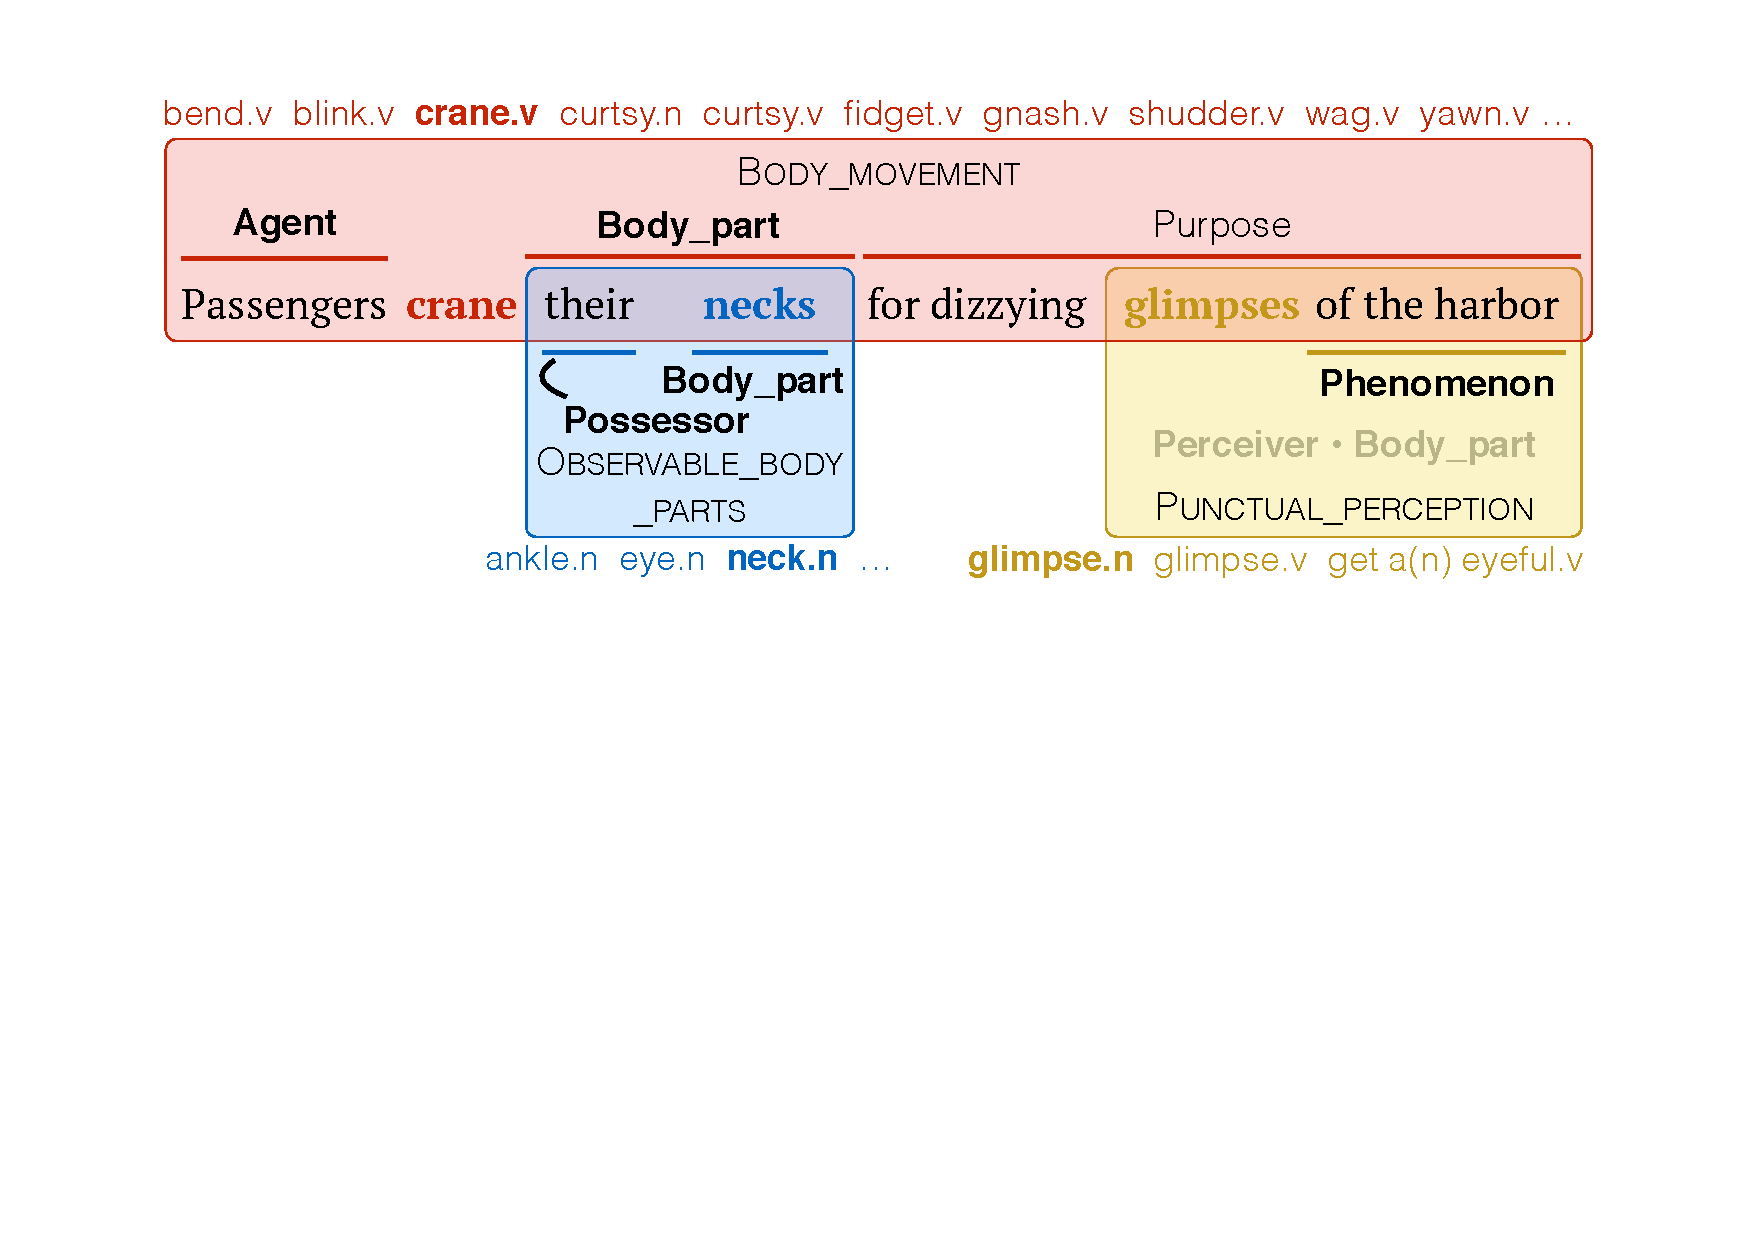
\includegraphics[width=\columnwidth]{fig/harbor-fn.pdf}
\caption{Example sentence from FrameNet full-text annotation. 
3~frames and their arguments are shown: 
\fnf{Body\_movement} is evoked by \textit{crane},
\fnf{Observable\_body\_parts} by \textit{necks}, 
and \fnf{Punctual\_perception} by \textit{glimpse}.
(Further, \textit{harbor} is annotated as evoking the \fnf{Locale\_by\_use} frame 
and doubles as its sole argument.) 
Horizontal lines representing argument spans 
are labeled with role names.}
\label{fig:harbor-fn}
\end{figure}

FrameNet~1.5 defines a structured hierarchy of over 1,000 frames associated with \nss{\#}~English lexical predicates, 
and also provides annotations for \nss{\# targets annotated total} attestations 
of these frames/predicates in corpora, annotated in context with their arguments. 
In FrameNet~1.5, a rather small number of sentences---\nss{\#}, comprising \nss{\#} words---% 
are provided with \textbf{full-text} annotations, i.e.~the sentence 
has been analyzed for all available frames. 
But a full \nss{\#}\% of sentences in FrameNet---the lexicographic \textbf{exemplars}---are annotated for only one frame per sentence, 
and have thus far not been exploited successfully for frame-semantic parsing.
Here, we seek to leverage these exemplar sentences 
as well as the (type-level) hierarchical structure of the FrameNet lexicon. 

\begin{figure}
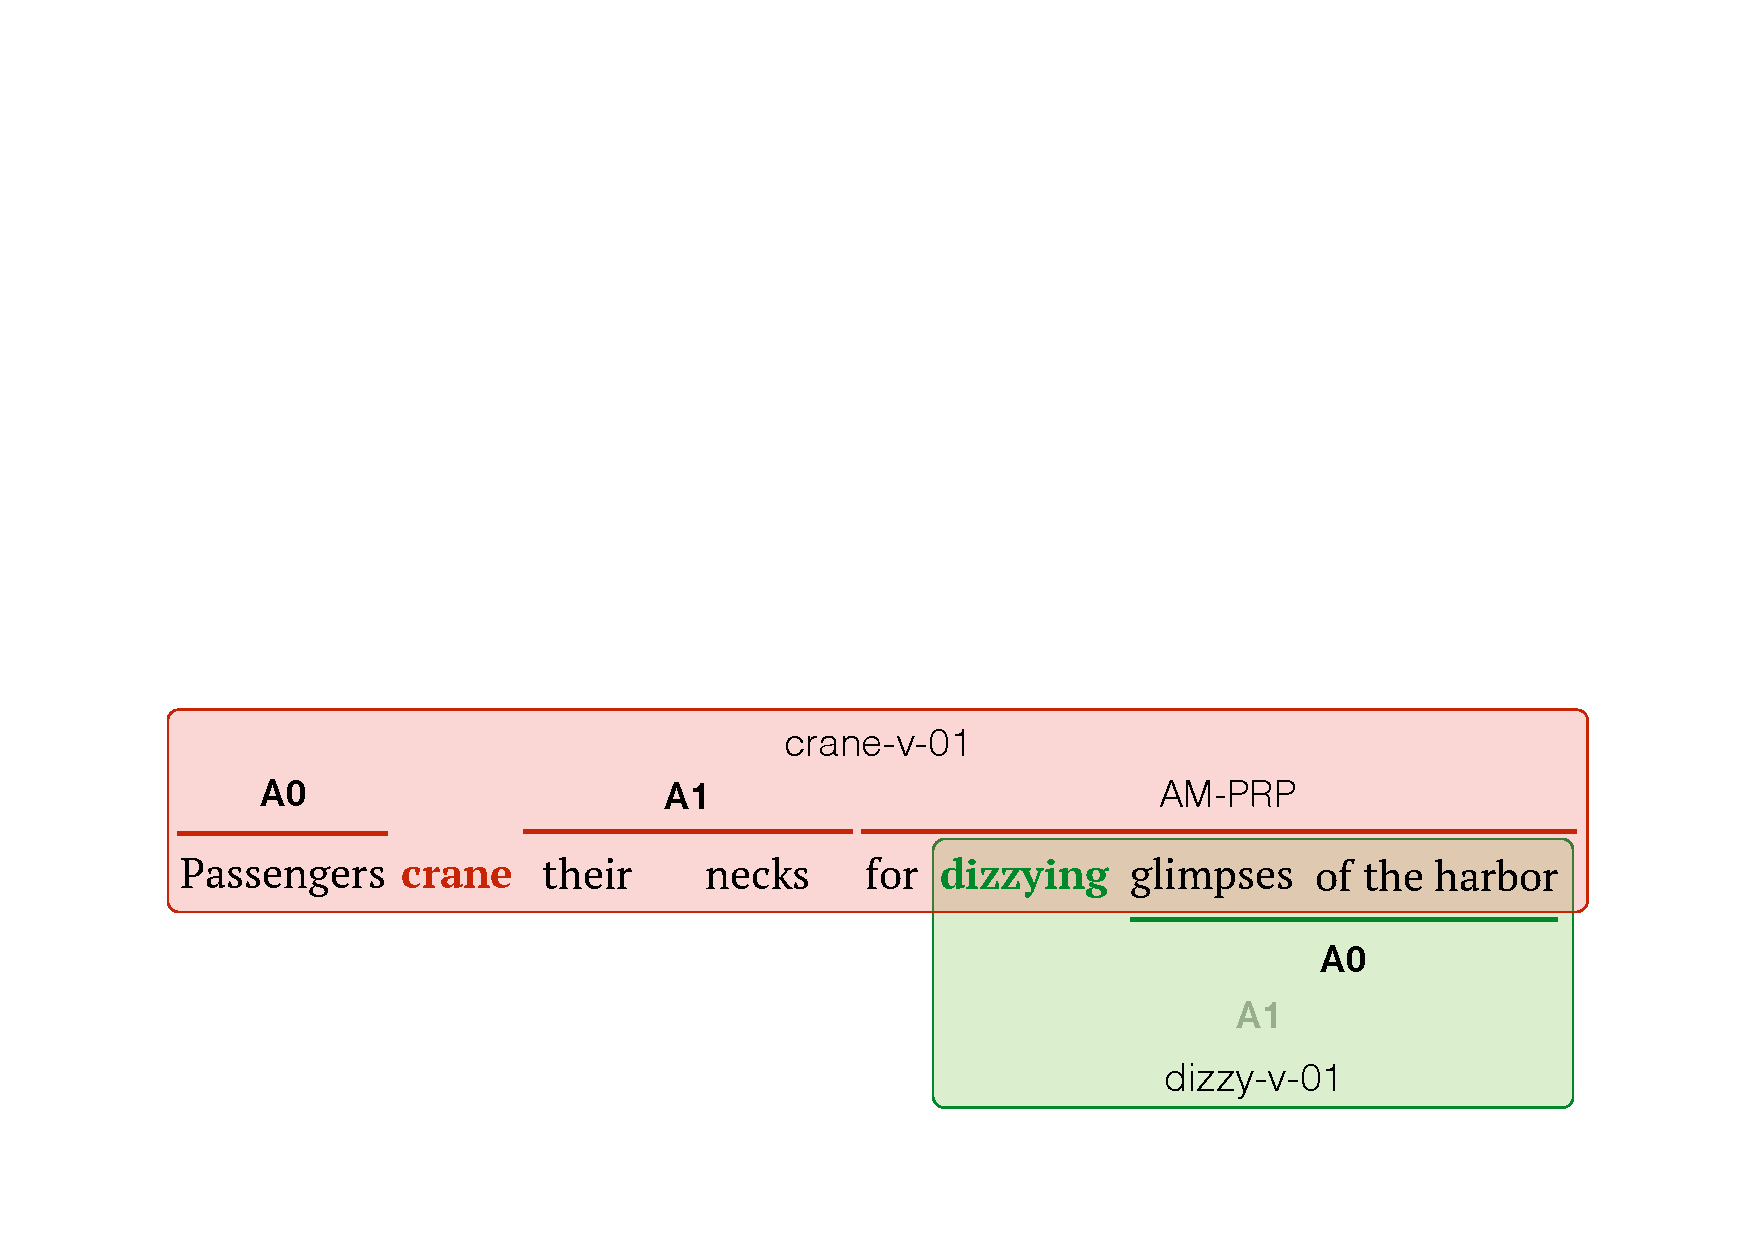
\includegraphics[width=\columnwidth]{fig/harbor-pb.pdf}
\caption{Ideal PropBank annotations for verbs. Though PB uses lexical frames rather than deep frames,
there are clear similarities to the FrameNet annotations in \cref{fig:harbor-fn}.}
\label{fig:harbor-pb}
\end{figure}

In this paper, we address the \textbf{argument identification} 
subtask of finding and labeling arguments 
given a predicate in context and the frame it evokes.
This is a form of semantic role labeling (SRL), 
a task introduced by \citet{gildea-02} using a much earlier version of FrameNet.
Notably, another resource, \textbf{PropBank} \citep{propbank}, has been widely used for SRL \citep{palmer-10}. 
PropBank annotations capture shallower lexical frames and arguments; 
additionally, PropBank provides \nss{millions?} of words of fully annotated English sentences
(annotation is much less expensive, but also potentially less valuable, because of the shallower representation).
Despite a number of differences in the representations and annotation conventions, 
for many predicates FrameNet and PropBank are really quite similar: 
\cref{fig:harbor-fn} and \cref{fig:harbor-pb} show this for the verb \textit{crane}.
To get the best of both worlds, we aim to tap into PropBank's vast resources 
as indirect token-level supervision for FrameNet-style analysis. 
We hypothesize that PropBank analyses can serve as a weak signal for the FrameNet SRL task, 
either by heuristically transforming PropBank annotations into FrameNet annotations 
to augment the training data, or by preprocessing sentences with a PropBank SRL system to obtain new features 
for FrameNet argument identification.

Our experiments expand the \emph{training data} and/or the \emph{feature space}
of supervised argument identification
in order to integrate evidence from all of these sources 
into SEMAFOR \citep{das-14}, the leading open-source frame-semantic parser for English.\footnote{\url{http://www.ark.cs.cmu.edu/SEMAFOR/}} 
The results show that some of these sources of evidence succeed 
at boosting argument identification performance.\nss{SOTA (without constraints)?}


\section{Resources}

\nss{incl. data analysis of differences from full-text}

\nss{w/in each mention: genre/overall vocabulary; coverage and distributions of predicates, FE labels; oracle coverage of FT test}

\subsection{The FrameNet Lexicon}\label{sec:lex}

Each frame in the Berkeley FrameNet lexicon is intended to represent a gestalt scene. 
The frame definition includes: a descriptive name; 
a set of \textbf{core roles} representing participants and props that are crucial 
to understanding the scene; a set of \textbf{non-core roles} such as circumstantial 
information (time, place, manner, purpose, etc.); 
an English textual description of the scene and how its roles relate to one another;
and a set of English predicates that can evoke the scene.
For example, the \fnf{Body\_movement} frame has \fnr{Agent} and \fnr{Body\_part} as its core roles; 
the frame description states,
``This frame contains words for motions or actions an \fnr{Agent} performs using some part of his/her body.''
Lexical entries in this frame include verbs such as \fnlu{bend}, \fnlu{blink}, \fnlu{crane}, and \fnlu{curtsy}, 
plus the noun use of \fnlu{curtsy}.

The frame lexicon is organized as a network, with several kinds of \textbf{frame-to-frame relations} 
linking pairs of frames and (subsets of) their arguments \citep{ruppenhofer-10}. 
Among these kinds of frame-to-frame relations are:
\begin{itemize}
\item \textbf{Inheritance:} E.g., \fnf{Punctual\_perception} (e.g., \fnlu{glimpse.v}) inherits from 
\fnf{Perception\_experience} (e.g., \fnlu{see.v}), which inherits from \fnf{Perception}. 
Other frames inheriting from \fnf{Perception} include \fnf{Sensation} (e.g., \fnlu{sight.n}) and 
\fnf{Becoming\_aware} (e.g., \fnlu{notice.v}). Crucially, roles in inheriting (conceptually more specific) frames are mapped 
where they correspond to a role in the inherited frame: so \fnf{Punctual\_perception}.\fnr{Perceiver} links to \fnf{Perception\_experience}.\fnr{Perceiver\_passive}, 
which links to \fnf{Perception}.\fnr{Perceiver}, which links to \fnf{Sensation}.\fnr{Perceiver\_passive} and \fnf{Becoming\_aware}.\fnr{Cognizer}.
\item \textbf{Subframe:} This indicates a subevent within a complex event. 
E.g., the \fnf{Criminal\_process} frame groups together subframes 
\fnf{Arrest}, \fnf{Arraignment}, \fnf{Trial}, and \fnf{Sentencing}. 
\fnf{Criminal\_process}.\fnr{Defendant}, for instance, is mapped to 
\fnf{Arrest}.\fnr{Suspect}, \fnf{Arraignment}.\fnr{Defendant}, 
\fnf{Trial}.\fnr{Defendant}, and \fnf{Sentencing}.\fnr{Convict}. 
Other salient participants in the complex event (such as the crime for which someone is arrested, 
tried, etc.)\ are similarly mapped via Subframe relations.
This permits an inference that a person tried for a crime likely
has been or will be arrested, arraigned, and sentenced for that crime.
\end{itemize}
In \cref{sec:hierfeats}, we experiment with features shared between related roles of related frames 
in order to capture statistical generalizations about the kinds of arguments 
seen in those roles and how they relate syntactically to the predicate.

\subsection{Full-text Annotations}\label{sec:ft}

Contemporary frame-semantic parsers are trained and evaluated on the \textbf{full-text (FT)}\footnote{Though these 
were \emph{annotated} and the document level, and train/dev/test splits are by document, the frame-semantic parsing 
is currently restricted to the sentence level.} portion 
of the FrameNet corpus. This consists of documents for which annotators made an effort 
to assign frames and arguments to as many words as possible. 
\Cref{fig:harbor-fn} gives an example sentence from the FT portion of the corpus. 
It has 4~frame annotations. \fnf{Body\_movement}, as described in the previous section, 
is evoked by \textit{crane}, and 3~of its roles are filled by overt arguments: 
the 2~core roles (\fnr{Agent}, \fnr{Body\_part}) happen to be filled by noun phrases 
(\textit{passengers}, \textit{their necks}), while the non-core role \fnr{Purpose} is filled by a 
prepositional phrase adjunct (\textit{for dizzying glimpses of the harbor}).
The frame defines 19~additional non-core roles, none of which have an argument in the example.
In frame semantics, non-core roles are considered to be \emph{conceptually} optional; 
core roles may or may not be \emph{syntactically} optional, but if not locally specified they are 
expected to be available from context, or else implicit.
For example, \fnf{Punctual\_perception}---evoked in this case by \textit{glimpses}---is annotated 
as missing 2~of its core roles. A human listener would resolve the identity of the \fnr{Perceiver} 
from the wider context and the \fnr{Body\_part} from world knowledge. 

In some cases, FT annotation involved creating a new frame or adding a new lexical unit to an existing frame. 
In other cases, words that in principle should be considered to evoke a frame were left unannotated 
because they did not match any existing lexical units. 
This was the case for \textit{passengers} and \textit{dizzying} in \cref{fig:harbor-fn}.

\nss{Genres, sizes}

\nss{Annotation density: (proportion of tokens evoking a frame. breakdown by POS?)}

\subsection{Exemplars}\label{sec:exemplars}

\nss{how different from FT}

\subsection{PropBank}\label{sec:pb}

PropBank \citep[PB;][]{palmer-05} is a lexicon and corpus of predicate--argument structures
that takes a shallower approach than FrameNet. Whereas FrameNet frames cluster 
lexical predicates that evoke similar kinds of scenarios (with the same kinds of roles), 
and these frames are organized in a network, 
PropBank frames are purely lexical and there are no formal relations between different predicates 
or their roles.
PropBank does represent lexical ambiguity---e.g., the verb \textit{order} is ambiguous 
in PropBank between \pbf{order-v-01} ``impelled action'' and \pbf{order-v-02} ``request to be delivered''---but
PropBank's sense distinctions are generally coarser-grained than FrameNet's.

Within sense-disambiguated PropBank frames, or \textbf{rolesets}, 
core roles are defined with textual descriptions and assigned numbers. 
E.g., \pbf{order-v-02} defines: \pbr{A0} ``orderer'', 
\pbr{A1} ``thing ordered'', \pbr{A2} ``benefactive, ordered-for'', 
and \pbr{A3} ``source''.
Following \citeposs{dowty-91} theory of proto-roles, PropBank rolesets use \pbr{A0} for proto-agents 
and \pbr{A1} for proto-patients, but in general, there is much less consistency 
in interpretation of core roles across lexical predicates for PropBank than there is for FrameNet.
Another difference is that PropBank's non-core roles---named \pbr{AM-*}, 
such as \pbr{AM-PRP} for purposes---are not frame-specific.\footnote{\Citet{ellsworth-04} 
has a more extensive discussion of differences between PropBank's and FrameNet's conventions.}

Despite all these differences, there is often a great deal in common between 
FrameNet-style and PropBank-style analyses, as should be apparent from comparing 
\cref{fig:harbor-fn} and \cref{fig:harbor-pb}. 
The major benefit to PropBank is that it includes a large and comprehensively annotated corpus.
We hypothesize that leveraging this large corpus indirectly 
can reap rewards for frame SRL. 

\subsection{Illinois SRL system}\label{sec:pbsrl}

\subsection{SemLink}\label{sec:semlink}

\nss{limitations!}





\section{Learning from multiple domains and representations}

We use the model from SEMAFOR \citep{das-14}, described in \S\ref{sec:base_model}, as a starting point.
We experiment with several domain adaptation techniques, augmenting the model's training data (\S\ref{sec:aug_data}) and feature space %$\mathbf{\phi}$
(\S\ref{sec:frust}--%,\ref{sec:frust},\ref{sec:guide},
\ref{sec:hierfeats}).
% modifying the model-fitting portion of the argument identification model's local learning objective  (training data, features).


\subsection{Base model}
\label{sec:base_model}

The argument identification task is treated as a structured prediction problem.
% We consider the argument identification task as statistical classification 
% for each role of the frame in context.
Let the classification input be a dependency-parsed sentence $\mathbf{x}$, 
the token(s) $p$ constituting the predicate in question, and the frame $f$ evoked by $p$
(as determined by frame identification). 
We use a heuristic procedure \st{cite} for extracting candidate argument spans 
for the predicate; call this $\textit{spans}(\mathbf{x}, p, f)$.
$\textit{spans}$ always includes a special span denoting an empty or non-overt role, denoted $\emptyset$. 
For each candidate span $a \in \textit{spans}(\mathbf{x}, p, f)$, we extract a binary feature vector 
$\mathbf{\phi}(a, \mathbf{x}, p, f)$.
We describe the features in \S\ref{sec:features}.
We use a linear model, parametrized by the weight vector $\mathbf{w}$, to score $a$:
\begin{equation}
\textit{score}_\mathbf{w}(a \mid \mathbf{x}, p, f, r) = \mathbf{w}^\top \mathbf{\phi}(a, \mathbf{x}, p, f, r)
\end{equation}
$\textit{score}_\mathbf{w}$ models the compatibility  of a candidate
role--argument pair, and its parameters (feature weights) $\mathbf{w}$ are
learned from data (\S\ref{sec:learning}).

At inference time, we use a \term{global classifier}.
The global classifier chooses a joint assignment of all arguments of a frame, while respecting the following constraints:
\begin{enumerate}
  \item a role may be assigned to at most one span, and
  \item spans of overt arguments must not overlap.
\end{enumerate}
Concretely, let a joint assigment be represented as a function $\mathbf{a}: \textit{roles}(f) \rightarrow \textit{spans}(\mathbf{x}, p, f)$, % \cup \{\emptyset\}$, %= \{ (r, a) \mid r \in \textit{roles}(f) \}$
 and let $\mathcal{A}$ be the set of all non-overlapping assignments.
We give $\mathbf{a}$ the score
\begin{equation}
\textit{score}_{\mathbf{w}}(\mathbf{a} \mid \mathbf{x}, p, f) =
    \sum_{r \in \textit{roles}(f)}{\textit{score}_\mathbf{x}(\mathbf{a}(r) \mid \mathbf{x}, p, f, r)}
\end{equation}
And choose the joint assignment
\begin{equation}
\textit{args}(\mathbf{x}, p, f) =
    \argmax_{\mathbf{a} \in \mathcal{A}} {
        \textit{score}_{\mathbf{w}}(\mathbf{a} \mid \mathbf{x}, p, f, r)
    }
\end{equation}
Beam search, with a beam size of 100, is used to find this $\argmax$.%
\footnote{Recent work has improved upon global decoding techniques \st{cite Täckström et al, TACL}.
We expect such improvements to be complementary to the gains due to the added features and data reported here.}

\mk{introduce this as a supervised domain adaptation problem? What is the source and what's the target?}
\mk{Let $D_{ft}$ represent the FT data and $D_{ex}$ the exemplars?}


\nss{Domain adaptation/multitask learning techniques}

\subsection{Augmenting the Training Data}
\label{sec:aug_data}

\subsection{Frustratingly Easy}
\label{sec:frust}
\cite{daume-2009} proposed a simple feature augmentation approach that was shown to work well in supervised domain adaptation scenarios, 
such as ours.
Let $\mathcal{D}_{FT}$ be the full text data, and $\mathcal{D}_{ex}$ be the exemplar data.
We %apply their method to incorporate the exemplars data  by introducing
introduce a domain feature $I_{\textit{domain}}(\mathbf{x}) = \indicator{\mathbf{x} \in \mathcal{D}_{FT}}$,
where $\indicator{\cdot}$ is the indicator function, \[
\indicator{P} = \left\{\begin{array}{lr}
1, & \text{ if } P \\
0, & \text{ otherwise}. \\
\end{array}
\right.
\]
We expand the feature space by concatenating the original feature vector with a version of the feature vector that has been element-wise conjoined with the domain indicator:
% We apply their method to incorporate the exemplars data  by introducing a feature mapping $\Phi : \mathds{R}^d \rightarrow \mathds{R}^{2d}$ given by
% \begin{equation}
% \Phi(\mathbf{\phi}(a, \mathbf{x}, p, f, r)) = [x; x * ]
% \end{equation}
%  for the
\begin{align*}
\lefteqn{
\phi_{\textit{frust}}(a, \mathbf{x}, p, f, r) =
} \\
&&
\left[\begin{array}{c}
\phi(a, \mathbf{x}, p, f, r) \\
\phi(a, \mathbf{x}, p, f, r) \text{ \& } I_{\textit{domain}}(\mathbf{x})
\end{array}
\right]
% \left[\phi(a, \mathbf{x}, p, f, r) ; \phi(a, \mathbf{x}, p, f, r) \wedge I_{\textit{domain}}(\mathbf{x}) \right]
\end{align*}


% FT annotations $x \in \mathcal{D}_{ft}$, and $\Phi^{ex}(x) = (x, 0)$ for the exemplars $x \in D_{ex}$. The resulting transformed data 
% from the two domains is then used to learn a single model.
The intuition is that by replicating the features, we allow for
each feature to contribute both ``general'' and ``domain-specific'' weights to the model depending on whether the feature
behaves similarly in both domains or not.
Since the general feature contributes to both domains, regularization will encourage the model to use the general version over the domain-specific version of a feature whenever possible.

\subsection{Guide Features}
\label{sec:guide}
Another approach to introduce supervision for domain adaptation, 
which does not combine the labeled data from the two domains, 
to use a supervised model built on the source domain to augment features in the target domain.
When training and testing in the target domain, 
the source domain model is effectively just a form of preprocessing to provide 
additional features, known as \textbf{guide features} \citep{johansson-13,kong-14}.\footnote{This is related to the technique
of model stacking, where successively richer models are trained by cross-validation on the same dataset 
\citet[e.g.,][]{cohen-05,nivre-08,martins-08}.}
Formally: let $M_{s}$ be the model built on
the source domain (for instance, the PropBank data). 
For every target instance $x$, we introduce ``guide'' features which use the output $M_s(x)$
obtained by applying $M_s$ on $x$, which consists of the role labels assigned to various text spans in $x$. 
Two types of guide features were used,
one to indicate that a span $s_x$ was assigned a role and the other encoding the role label $r_g$ itself. 
In the case where $M_s$ produces labels
that belong to the same schema as the target domain 
(for instance, the exemplars use the same schema as the FT annotations), 
we use an additional feature $f_{match}(r_t,r_g)$ to indicate that 
the `guide' role label $r_g$ of the span $s_x$ is the same as it's true label $r_t$.


\subsection{Type-level hierarchy features}\label{sec:hierfeats}
\mk{NSS: notation for the frame/role/features etc?}
\mk{How many total types of relations? Cleanup writeup based on NSS's notation.}

Frames in FrameNet are connected to each other by relations such as inheritance, temporal ordering, causality. 
For instance, the frame \fnf{Robbery} inherits from the more abstract frame \fnf{Committing\_crime}, and the
frame \fnf{Fall\_asleep} is preceeded by the frame \fnf{Being\_awake}. The roles of related frames have 
also been mapped to indicate the correspondence between them: \fnf{Robbery}.\fnr{Perpetrator} is mapped to 
\fnf{Committing\_crime}.\fnr{Perpetrator}, which in turn maps to \fnf{Misdeed}.\fnr{Wrongdoer}. Frames and roles that are far
apart in this hierarchy are less related than say neighbours.
This hierarchy can be exploited to share information across related roles, thereby benefiting the roles 
that have few annotations \mk{say something about a greater variety of contexts is available for each role}. 
We say that the $\textit{parent}$ of a role is one that has either the \textbf{Inheritance} or \textbf{Subframe} relation to it (\cref{sec:lex}).
There are 4138 \textbf{Inheritance} and 589 \textbf{Subframe} links between role types in FrameNet 1.5.

A simple mechanism to share information is via shared model parameters between related roles. Towards this, we experiment with two variations of
hierarchical feature types:

\noindent\textbf{(1) siblings}: Roles that have a common parent share features.
For every feature $\phi_i(a, \mathbf{x}, p, f, r)$, we add a new feature which is the conjunction: 
$\text{"sib"} \wedge \phi_i(a, \mathbf{x}, p, f, r) \wedge \textit{parent}(r)$. 
% $I_{hier}$ is an indicator to distinguish this feature from the regular conjunction features in Semafor that use frame names and roles.

\noindent\textbf{(2) parent+siblings}: Roles share features with their parent and siblings. 
For every feature $\phi_i(a, \mathbf{x}, p, f, r)$, we add a two new features:

\noindent$\text{"par+sib"} \wedge \phi_i(a, \mathbf{x}, p, f, r) \wedge \textit{parent}(r)$, and

\noindent$\text{"par+sib"} \wedge \phi_i(a, \mathbf{x}, p, f, r) \wedge r$.

We experimented with using more than one level of the hierarchy (grandparents, e.g.), but found that it does not produce any improvements in the performance, yet increased computation cost due to the greater number of features.

\mk{Write about the number of features in all models somewhere.. 
Baseline: 2709128, Combined training: 12972404, Frust-easy: 15681531, 'Parents+siblings': 34282958}

\section{Experiments}

All of our experiments use the same form of regularization, 
condition on the same oracle frame predictions, 
and syntactic preprocessing\nss{does this match Dipanjan's latest experiments?}, 
and use beam search with a beam size of 100 for joint decoding of the test data.
Automatic syntactic dependency parses from MSTParserStacked \citep{martins-08} are used, as in \cite{das-14}. % to narrow the set of candidate spans considered, and as input to feature extraction.


\subsection{Learning}
\label{sec:learning}

\st{TODO: local classifier is only used in my SVM version, not in Das's log-linear version.}
We define the \textbf{local classifier} as:
\begin{equation}
\textit{arg}(\mathbf{x}, p, f, r) = \argmax_{a \in \textit{spans}(\mathbf{x}, p, f)%\cup \{\emptyset\}
} \textit{score}_{\mathbf{w}}(a \mid \mathbf{x}, p, f, r)
\end{equation}
% This is used to choose an argument for every role $r$ of frame $f$.
We use the local classifier during training.

\st{talk about learning here?}
\st{something about L2 regularization}


% SEMAFOR treats the argument identification task as a structured prediction problem.
% It uses a linearly parametrized model that scores each candidate span given a frame element\st{this should probably be talked about earlier?}:
% \begin{equation}
% \textit{score}_\mathbf{w}(y \mid x) = \mathbf{w}^\top \mathbf{f}(x, y)
% \end{equation}

% During training, each frame element is treated as an independent log-linear classification instance, with the set of candidate spans (including the \textsc{NULL} span) as its output space.
% \st{something about L2 regularization}
% But at test time, it chooses a joint assignment of all arguments that maximizes probability under the model, while satisfying the following constraints:
% \begin{enumerate}
%   \item an argument may be assigned to at most one span \st{theta criterion, Chomsky}, and
%   \item spans of realized arguments must not overlap.
% \end{enumerate}
% Beam search, with a beam size of 100, is used to choose the maximum joint assignment with no overlapping arguments.
% \nss{does beam search require normalizing to probabilities?}\st{no. maybe it should, but SEMAFOR didn't, and we don't.}

We have made several modifications to SEMAFOR's training in order to speed up experiments:

\begin{itemize}
  \item We use squared structured hinge loss (defined below) instead of multiclass logistic regression.
  Using hinge loss, there is no longer a need to calculate a partition function.
  Gradients, and hence parameters, are sparser than in logistic regression, allowing us to use a sparse vector implementation.
  \item We use the online optimization method AdaDelta \citep{zeiler-12} with minibatches\nss{minibatch size?}, instead of the batch method L-BFGS \citep{liu-89}.
%   \item We use elastic net ($\ell_1 + \ell_2$) regularization. Adding $\ell_1$ also has the effect of keeping the parameter vector sparse.\nss{what hyperparameter(s)? are $\ell_1$ and $\ell_2$ tuned separately?}
\end{itemize}
We use these changes for all systems, including the baseline.
While the impact on full-text performance is negligible, 
these changes enabled us to run more experiments with the larger exemplar dataset and expanded feature space.\footnote{With SEMAFOR's original features and training data, 
the result of the above changes is that full-text $F_1$ decreases from 59.3\% to 59.1\%, 
while training time (running optimization to convergence) 
decreases from 729 minutes to 82 minutes\nss{say something about hardware this was tested on?}.%
%\mk{P/R/F numbers are in the table (see rows 1 and 2). Times: 12 hrs 9 mins for the earlier algorithm to converge. That took 290 iterations. An equivalent number of iterations took 45 minutes for the new system. Running till convergence (about 700 iterations) took 82 minutes, thus giving a speed-up of $\approx$ 9X. The P/R/F on exemplars improves (row 2); I believe it is due to the regularization in Sam's objective.}
} 


The details of squared hinge loss are as follows.
Let $(x^{(i)}, y^{(i)})$ be the $i^{\text{th}}$ training example.
Then the structured hinge loss on the $i^{\text{th}}$ example is given by:
\begin{align*}
\lefteqn{\textit{Hinge}_\mathbf{w}(i) =} \\
&&\max_y{\{\mathbf{w}^\top \mathbf{f}(x^{(i)}, y) + \text{cost}(y, y^{(i)})\}} - \mathbf{w}^\top \mathbf{f}(x^{(i)}, y^{(i)})
\end{align*}
and squared hinge loss is:
\begin{equation}
\textit{SquaredHinge}_\mathbf{w}(i) =
\textit{Hinge}_\mathbf{w}(i)^2.
\end{equation}
In our experiments, we use $\text{cost}(y, y^{(i)}) = \indicator{y \ne y^{(i)}}$ \st{define}\footnote{We experimented with recall-oriented training, where errors of omission are assigned a higher cost, but found that while recall increased, overall $F_1$ went down\nss{or: failed to improve?}.}.


\nss{same FN 1.5 splits as Dipanjan}


\nss{preprocessing issues: removing duplicate sentences, merging adjacent split args in exemplars, OntoNotes PropBank preprocessing (NLTK), token-level SemLink details (such as filtering out sentences without mappable annotations; copy from WS paper)}

\subsection{Preprocessing the data}


\mk{NSS: hope you're not duplicating this in the earlier section! 
We use the \emph{token-level parallel annotations} from SemLink, which are available for a subset of the PB-WSJ text, 
hereafter referred to as SL-WSJ.} Of the available 74,977 SL-WSJ verbs, a majority cannot be mapped to FN frames for various reasons.
Around 31\% of the predicates have the frame label \texttt{IN} (``indefinite'') where the mapping from VerbNet to FrameNet is ambiguous.
About 20\% of the instances are labeled \texttt{NF} (``no frame''), indicating a coverage gap in FrameNet. 
21\% of verbs have frame labels but no frame element annotations. Most of these are predicates with modifier arguments.
Other arguments pointed to null anaphora that could not be resolved to overt arguments.
This leaves 15,323 mappable instances with at least one overt argument, or 20\% of SL-WSJ verbs. This is a very small
subset of the entire PB annotated data.

We processed the exemplars data to remove duplicate sentences that already appear in the FT data. 



\nss{tuning regularizer for all experiments}
We tune the $\ell_2$ regularization parameter $\lambda$ on the held-out set. We searched over the following
values: 10$^{-5}$, 10$^{-7}$, 10$^{-9}$, 10$^{-12}$ (note that our loss is normalized).
We also use the performance on the held-out set to determine the stopping criterion for the stochastic optimization.




\subsection{Evaluation}
The argument identification performance of the various methods is compared on two different test sets.
(1) Full-text: the FrameNet 1.5 FT test split that was used in the evaluation in \cite{das:2012}. This data consists of sentences from 23 documents. 
(2) Exemplars: a randomly sampled set of sentences from the exemplars data, with approximately the same number of targets as the FT test set.
Statistics of both the test sets are given in the lower half of Table \ref{tbl:datastats}. 
The FT test set has 289 unseen role types, which is much higher than
the 38 in the exemplars test set. There are no unseen frame types in the exemplars test data, whereas the FT test has 46 of them. 
These differences are due to the manner in which the train and test splits were created, with document-level splits being used
for FT and sentence-level splits for the exemplars.
The last row of Table \ref{tbl:datastats} shows the unseen role types faced by a model that was built on both the FT and exemplars training data.
In the FT test set it is 103, lower by $\approx$190 than what a FT-only model will see, thus leading us to expect that a model that combines
both sets of data will certainly benefit in performance.


\begin{table}\centering\small
\begin{tabular}{p{4cm}rr}
\toprule
\normalfont & \textbf{Full-Text} & \textbf{Exemplars} \\
\midrule
Sentences in training & 2,780 & 145,838 \\
Roles in train data & 15,019 & 137,511 \\
Roles (types) in training & 2,644 & 4,821 \\
Sentences in test data & 2,420 & 4,132 \\
Roles in test data & 4,458 & 4,132 \\
Roles (types) in test data & 1,420 & 1,224 \\
Unseen frames (types) in test data & 46 & 0 \\
Roles (types) in unseen frames & 178 & 0 \\
Unseen roles (types) in test data & 289 & 38 \\
Unseen roles (types) in test w.r.t (FT+Exemplars) & 103 & 32 \\
\end{tabular}
\caption{Characteristics of the training and test data}
\label{tbl:datastats}
\end{table}

While the FT test set represents the benchmark set for evaluating the 
performance of a frame semantic role labeling system, the exemplars test set being from a different distribution of text, gives us
an indication of how well a model generalizes.

\subsection{Results}

\nss{results table without hierarchy features}

\nss{hierarchy features: which ones work best (decided on baseline), how do they improve best result so far}

\nss{Sam's curves on per-FE $F_1$}

\nss{comparison to prior work (baseline, best result). args+frames score vs. args only}

\nss{discussion throughout}

We present precision, recall, and F1-measure microaveraged across the test instances in Table \ref{tbl:results}, for all the approaches that we tried.
The first column classifies the approaches based on what resource we use and the second column indicates what training data was used. 
For each resource (one multi-row in the table) we show results obtained by various methods of combining it with the FT data.
The $\xrightarrow{\text{guide}}$ refers to the feature augmentation discussed in Section \ref{sec:guides},
`Hier' represents the hierarchical features from Section \ref{sec:hier} and `EasyAdapt' is described in Section \ref{sec:frust-easy}.

To summarize the results, we find that adding the sibling-level hierarchical features, using Exemplars as gold-standard training data and 
incorporating PB-SRL data in the form of guide features all help in improving the performance over the baseline on both FT-test and exemplars-test.

\begin{table*}\centering\small
\begin{tabular}{>{\itshape}clr<{\hspace*{15pt}}rrr@{~~}r@{~~}rrr}
\toprule
\normalfont\textbf{Additional} & \multicolumn{1}{c}{\textbf{Training Configuration}} & \multicolumn{1}{c}{\textbf{Millions of}} & \multicolumn{3}{c}{\textbf{Full-Text}} && \multicolumn{3}{c}{\textbf{Exemplars}} \\
\cline{4-6}\cline{8-10}
\normalfont\textbf{Resource} &  \multicolumn{1}{c}{\textbf{(Features)}} & \multicolumn{1}{c}{\textbf{Features}} & P\hphantom{11} & R\hphantom{11} & $F_1$\hphantom{0} && P\hphantom{11} & R\hphantom{11} & $F_1$\hphantom{0} \\
\midrule
%(Baseline) & FT (Basic) & 66.03 & 53.79 & 59.29 && 64.90 & 33.60 & 44.27 \\
(Baseline) & FT (Basic) & 2.7 & 65.57 & 53.82 & 59.12 && 62.63 & 37.65 & 47.03 \\
\midrule
\multirow{2}{*}{FN Hierarchy} & FT (siblings) & 5.4 & 67.24 & 54.76 & 60.36 && 64.81 & 39.09 & 48.77 \\
          & FT (siblings+parents) & 8.5 & 67.67 & 52.79 & 59.31 && 65.25 & 38.18 & 48.18 \\
\midrule
\multirow{2}{*}{SemLink} & SemLink $\xrightarrow{\text{guide}}$ FT & 3.0 & 64.67 & 54.53 & 59.17 && 60.95 & 38.92 & 47.50 \\
& FT+SemLink & 5.0 & 65.50 & 37.80 & 47.90 && 57.15 & 20.80 & 30.50 \\
\midrule
& Exemplars $\xrightarrow{\text{guide}}$ FT & 3.5 & 65.24 & 55.96 & 60.24 && 67.71 & 48.08 & 56.23\\
Exemplars & FT+Exemplars (Basic) & 13\nss{.?} & 66.06 & 58.23 & 61.90 && 75.44 & 65.11 & \bf{69.89} \\
& FT+Exemplars (EasyAdapt) & 16\nss{.?} & 65.70 & 59.04 & \bf{62.19} && 73.88 & 61.40 & 67.06 \\
\midrule
PB-SRL & PB-SRL $\xrightarrow{\text{guide}}$ FT & 3.6 & 64.96 & 54.83 & 59.47 && 61.38 & 39.14 & 47.80 \\
\bottomrule
\end{tabular}
\caption{Results on two test sets: Baseline vs.~individual other resources. 
Precision, recall, and $F_1$ are given as percentages.}
\label{tbl:results}
\end{table*}

\begin{table*}\centering\small
\begin{tabular}{lr<{\hspace*{15pt}}rrr@{~~}r@{~~}rrr}
\toprule
\multicolumn{1}{c}{\textbf{Training Configuration}} & \multicolumn{1}{c}{\textbf{Millions of}} & \multicolumn{3}{c}{\textbf{Full-Text}} && \multicolumn{3}{c}{\textbf{Exemplars}} \\
\cline{3-5}\cline{7-9}
\multicolumn{1}{c}{\textbf{(Features)}} & \multicolumn{1}{c}{\textbf{Features}} & P\hphantom{11} & R\hphantom{11} & $F_1$\hphantom{0} && P\hphantom{11} & R\hphantom{11} & $F_1$\hphantom{0} \\
\midrule
FT+Exemplars (Hier: siblings) & 34 & 66.00 & 60.40 & \bf{63.07} && 76.14 & 67.71 & \bf{71.70} \\
PB-SRL $\xrightarrow{\text{guide}}$ FT+Exemplars & 17 & 67.36 & 58.79 & 62.80 && 77.15 & 65.47 & 70.83 \\
%FT+Exemplars (PB-SRL, Hier: siblings) \\
\bottomrule
\end{tabular}
\caption{Combining best techniques across resources \nss{TODO}}
\label{tbl:bestTech}
\end{table*}


Consulting the results in detail, adding the sibling-level hierarchical features to the baseline FT model improves 
the fscore by 1.2 and 1.7 points on FT-test and exemplars-test respectively,
with benefits to both precision and recall. The (siblings+parents) features which consider two levels of the hierarchy produce unnoticeable benefits,
suggesting that higher levels in the hierarchy can be too general \mk{give example?}, resulting in very dissimilar roles firing the same hierarchy features.
\footnotetext{We also tried adding grand-parents and found only minor improvements. Using an expert-pruned hierarchy with relations that are
most likely to help can give greater benefits, and is beyond the focus of this work.}

SemLink, as we remarked earlier is a noisy resource and we see a confirmation for this observation in the performance of the (FT+SemLink) model,
which drops the f-score by a whopping 11.2 and 16.5 points below baseline on FT-test and exemplars resp. The guide features however modulate the influence
of the SemLink annotations, giving a minor increase over the baseline. 
%\mk{resulting in a graceful but prompt exit for this resource from further consideration.}

With the exemplars resource, we find that the guide features give us a modest improvement of 1.12 in F1 on FT-test, 
while using it as gold-standard training data results in a bigger increase of 2.8 points. 
On the exemplars-test we observe a similar trend, where the (FT+Exemplars) model delivers a massive increase of $\approx$23 f-points and a 
much smaller increase is seen with the guide features. This contrasts with what we observed for SemLink.
The frustratingly easy domain adaptation approach to incorporate the Exemplars
further improves the F1 by a minor 0.3 on the FT-test and a decent 2.8 on the exemplars-test.

Finally, using the PB-SRL data in the form of guide features also results in small improvements over the baseline. Overall we observe that an
additional resource that is very similar to the original resource helps more as training data than as a `guide model'.
Whereas the guide features help more when the additional resource is either unreliable (like SemLink) or too distinct (like PB). 

\mk{Analyze the sparsity of the models? Which features have highest importance?}
In addition to the performance, we also show the sizes of the various models in the column `number of features'. All the models are quite sparse however,
with $\approx$60-70 \% of the features assigned a zero weight. The larger models are also a lot slower to train, taking about 6 times
as long as the baseline. 

\begin{figure}[t]
	\begin{subfigure}[b]{0.5\textwidth}
		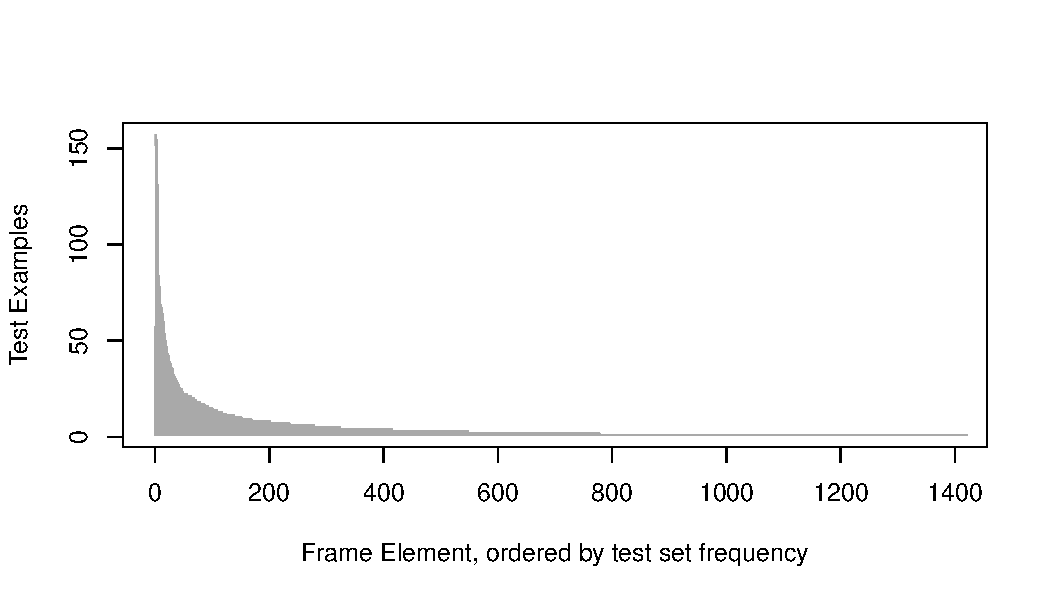
\includegraphics[width=\textwidth]{fig/num_instances}
	\end{subfigure}
	\begin{subfigure}[b]{0.5\textwidth}
		\vspace{-1cm}
		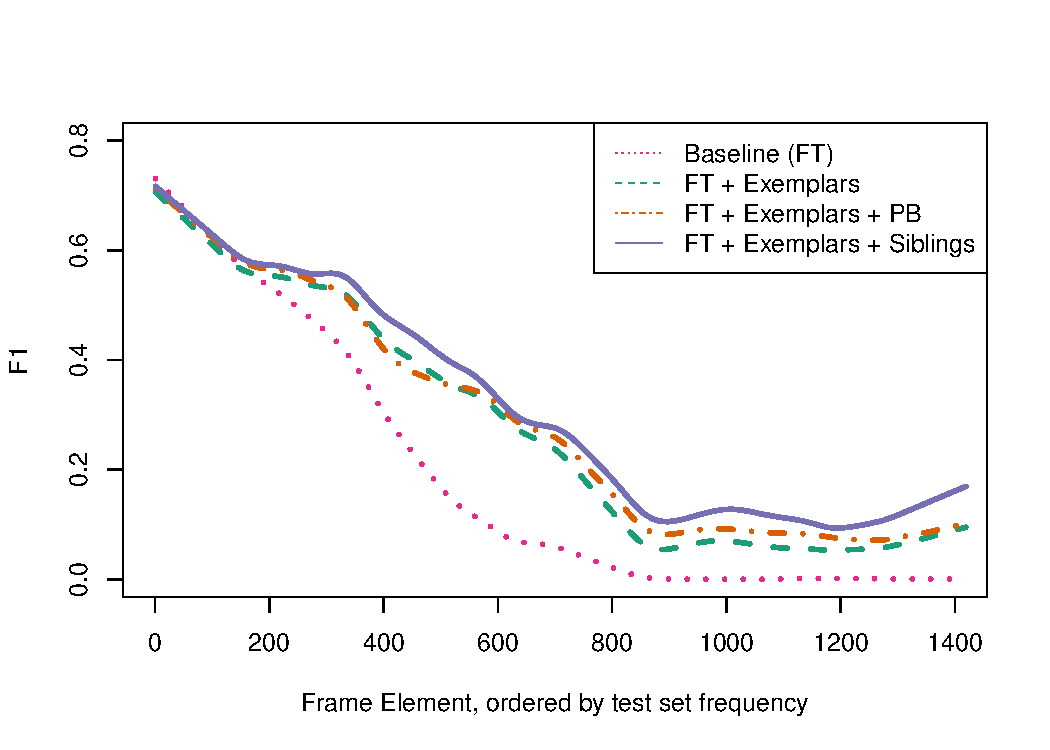
\includegraphics[width=\textwidth]{fig/f1_sorted_by_num_instances}
	\end{subfigure}
	\caption{Count and $F_1$ for each frame element appearing in the test set. $F_1$ values have been smoothed with \texttt{loess}, with a smoothing parameter of 0.2.}
\end{figure}


\section{Related Work}

\nss{Dipanjan's other papers; mention other PB SRL work?; anything using SemLink or combining resources for SRL? see \citep[\S4]{bonial-13}}

\nss{be sure to cite: \citep{shi-05} (multiple resources), \citep{matsubayashi-09} (hierarchy)}

\nss{multitask learning?}

\section{Conclusion}

\nss{overall findings}

\nss{future work: testing ground for improvements to PB \citep{bonial-14} and SemLink \citep{bonial-13}; automatic mappings between resources}

\finalversion{\section*{Acknowledgments}

FUNDING}

\smaller

\bibliographystyle{style/aclnat}
% you bib file should really go here
\setlength{\bibsep}{1pt}
{\fontsize{10}{12.25}\selectfont
\bibliography{argid}}

\end{document}
